\section{Results: dispersion, band gaps, and wave steering}
\label{sec:results}

The homogeneous isotropic solid serves as the reference for the orientation and aspect-ratio sweeps. The results then address the periodic composite, group-velocity steering and the high-wavenumber response. Case~H contains no periodic material contrast. Its positive $\Delta_{GX}$ values describe reduced-zone spectral separations, not Bragg attenuation gaps. Case~C contains periodic contrast and is examined separately for complete-gap formation. Unless otherwise stated, every reported Case-H directional and complete-gap measure ($\Delta_{GX}$, $\Delta_{XM}$, $\Delta_{MG}$, $\Delta_{\mathrm{path}}$, $\Delta_{\mathrm{complete}}$) is evaluated on the Bands~2--3 pair. The full parameter set is included in Appendix~\ref{app:parameter_summary}.

\subsection{Homogeneous isotropic baseline}
At $\mathrm{AR}=1$, the principal characteristic lengths coincide and the rotated length tensor is isotropic, so its constitutive response is independent of $\theta$. It therefore provides the reference for the anisotropic calculations, and Figure~\ref{fig:caseH_dispersion} plots its branches alongside theirs; its $\Gamma$--$X$ directional width is $\Delta_{GX}=0.041$.

\subsection{Anisotropy reshapes the Case-H branches}
Figure~\ref{fig:caseH_dispersion} compares the isotropic reference with two orientations of the anisotropic length tensor. Both acoustic branches start at zero frequency at $\Gamma$. Changing aspect ratio and orientation shifts the branches and lifts symmetry-related degeneracies at the zone edge. At $\mathrm{AR}=10$ and $\theta=45^\circ$, a narrow reduced-zone spectral separation appears along $\Gamma$--$X$, with $\Delta_{GX}=0.0043$. Modes propagating in other directions overlap this interval, so it is not a complete gap; the full-zone measure remains $\Delta_{\mathrm{complete}}\le -0.3235$.

In this model, the rotated length tensor changes the gradient-stiffness contribution according to propagation direction. The resulting branch shifts are therefore not uniform across the Brillouin zone: adjacent bands can separate along $\Gamma$--$X$ while modes at other wave vectors remain in the same frequency interval.

\begin{figure*}[htbp]
\centering
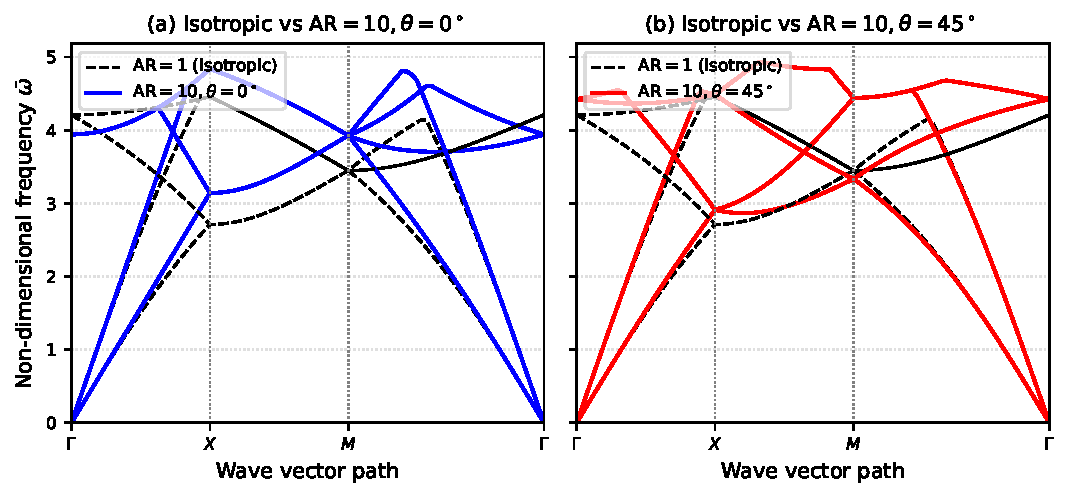
\includegraphics[width=\textwidth]{figures/fig06_caseH_dispersion.pdf}
\caption{Case-H Bloch bands along $\Gamma$--$X$--$M$--$\Gamma$. (a) Isotropic reference ($\mathrm{AR}=1$) and aligned anisotropy ($\mathrm{AR}=10$, $\theta=0^\circ$). (b) Isotropic reference and diagonal anisotropy ($\mathrm{AR}=10$, $\theta=45^\circ$), which opens a narrow $\Gamma$--$X$ reduced-zone spectral separation but no complete gap}
\label{fig:caseH_dispersion}
\end{figure*}

\subsection{Aspect-ratio and orientation effects}
At $\mathrm{AR}=5$, rotating the tensor from $0^\circ$ to $90^\circ$ lowers the transverse frequency at $X$ from $2.915$ to $2.672$ and the longitudinal frequency from $5.050$ to $4.628$ (Figure~\ref{fig:theta_sweep}). The projected gradient length changes from the major to the minor direction. The $M$-point frequencies are symmetric about $45^\circ$, as expected from the square-cell symmetry.

\begin{figure*}[htbp]
\centering
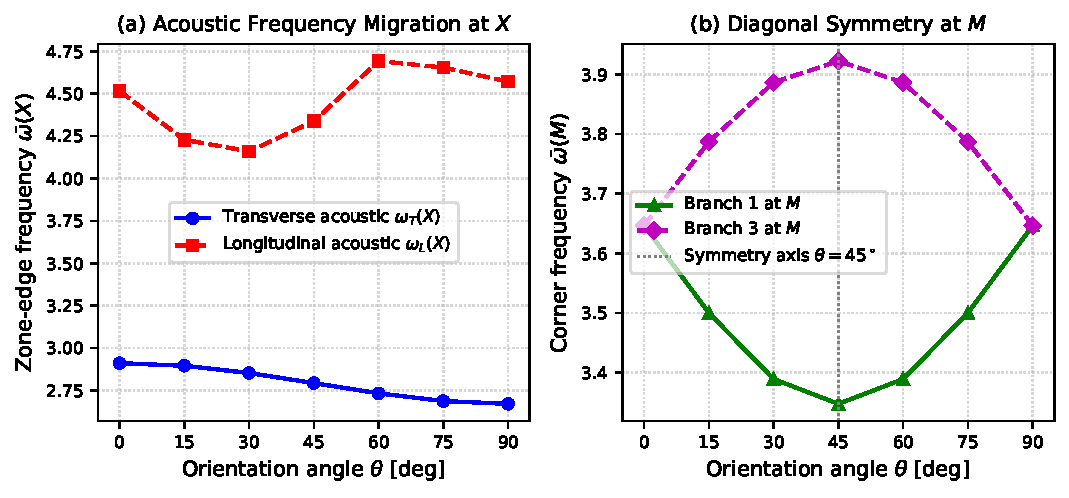
\includegraphics[width=\textwidth]{figures/fig08_theta_sweep.pdf}
\caption{Orientation dependence of the first four Case-H eigenfrequencies at (a) $X$ and (b) $M$ for $\mathrm{AR}=5$. The $M$-point response is symmetric about $\theta=45^\circ$}
\label{fig:theta_sweep}
\end{figure*}

Figure~\ref{fig:ar_sweep} isolates elongation at fixed $\theta=45^\circ$, using volume-equivalent length scaling. At fixed volume-equivalent length, increasing $\mathrm{AR}$ enlarges one principal length and reduces the other. The two band edges consequently respond differently, producing the non-monotone separation seen in the sweep.

\begin{figure*}[htbp]
\centering
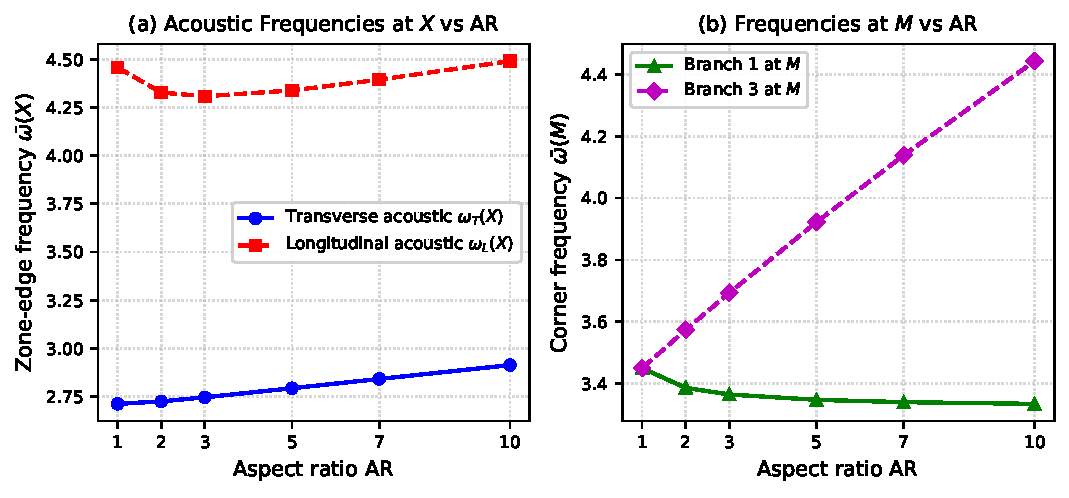
\includegraphics[width=\textwidth]{figures/fig09_ar_sweep.pdf}
\caption{Case-H branch frequencies at $X$ and $M$ as the aspect ratio varies from $1$ to $10$ at fixed $\theta=45^\circ$, using volume-equivalent length scaling}
\label{fig:ar_sweep}
\end{figure*}

\subsection{Directional spectral separation}
The $\Gamma$--$X$ interval is not empty of modes over the entire Brillouin zone. For example, at $\mathrm{AR}=10$ and $\theta=45^\circ$, $\Delta_{GX}=0.0043$ but the complete-gap measure is negative. No homogeneous configuration listed has a complete gap. Table~\ref{tab:gap_summary} lists representative gap measures; mesh-to-mesh variations are given in Appendix~\ref{app:numerical_checks}.

\subsection{Design-map interpretation}
The largest $\Delta_{GX}$ among the 42 sampled designs is $0.0677$ at $(\theta,\mathrm{AR})=(0^\circ,7)$ (Figure~\ref{fig:design_map}). Its dependence on aspect ratio is not monotone. The surface is an interpolation of these designs, not evidence of a continuously optimized configuration. Figure~\ref{fig:polar_map} groups the samples by the sign of $\Delta_{GX}$. The orientation sensitivity $S_\theta$ is largest at $\mathrm{AR}=10$ ($2.34\,\mathrm{rad}^{-1}$).

\begin{figure*}[htbp]
\centering
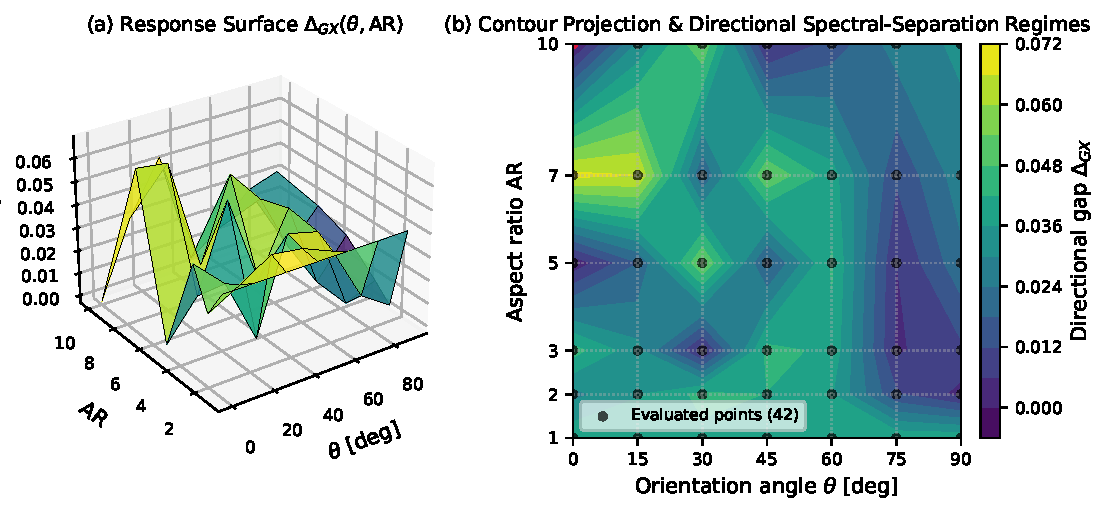
\includegraphics[width=\textwidth]{figures/fig10_design_map_3d.pdf}
\caption{Sampled Case-H design response $\Delta_{GX}(\theta,\mathrm{AR})$ for 42 configurations. The largest sampled value is $0.0677$ at $\theta=0^\circ$, $\mathrm{AR}=7$; at $\theta=45^\circ$, $\mathrm{AR}=10$, $\Delta_{GX}=0.0043$}
\label{fig:design_map}
\end{figure*}

\begin{figure*}[htbp]
\centering
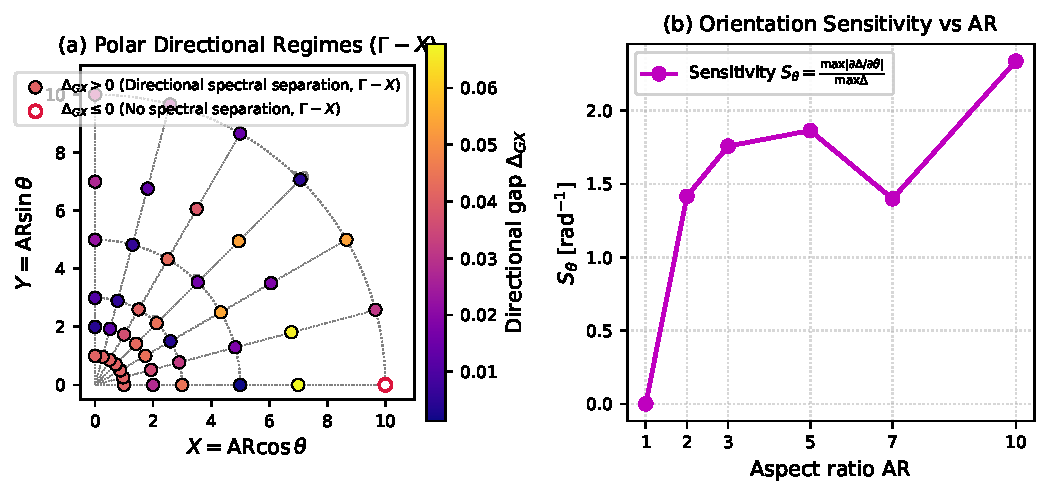
\includegraphics[width=\textwidth]{figures/fig11_polar_map_regimes.pdf}
\caption{Polar-coordinate view of the sampled Case-H designs, classified by $\Delta_{GX}\le0$ (pass band) and $\Delta_{GX}>0$ (directional spectral separation). The displayed boundary is a visual summary of sampled points}
\label{fig:polar_map}
\end{figure*}

\begin{table}[htbp]
\centering
\caption{Directional and complete-gap measures for representative Case-H configurations; values are reported at the precision retained between the $8\times8$ and $16\times16$ meshes}
\label{tab:gap_summary}
\begin{tabular*}{\textwidth}{@{\extracolsep{\fill}}c c r r r@{}}
\toprule
$\mathrm{AR}$ & $\theta$ & $\Delta_{GX}$ & $\Delta_{\mathrm{path}}$ & $\Delta_{\mathrm{complete}}$ \\
\midrule
$1$ & $0^\circ$  & $+0.041$ & $-0.32$ & $-0.32$ \\
$1$ & $45^\circ$ & $+0.041$ & $-0.32$ & $-0.32$ \\
$1$ & $90^\circ$ & $+0.041$ & $-0.32$ & $-0.32$ \\
$3$ & $0^\circ$  & $+0.045$ & $-0.10$ & $-0.46$ \\
$3$ & $45^\circ$ & $+0.044$ & $-0.45$ & $-0.48$ \\
$3$ & $90^\circ$ & $+0.011$ & $-0.33$ & $-0.46$ \\
$5$ & $0^\circ$  & $+0.001$ & $-0.01$ & $-0.58$ \\
$5$ & $45^\circ$ & $+0.016$ & $-0.48$ & $-0.58$ \\
$5$ & $90^\circ$ & $+0.022$ & $-0.37$ & $-0.58$ \\
$10$ & $0^\circ$  & $-0.002$ & $-0.24$ & $-0.85$ \\
$10$ & $45^\circ$ & $+0.004$ & $-0.29$ & $-0.56$ \\
$10$ & $90^\circ$ & $+0.031$ & $-0.65$ & $-0.85$ \\
\bottomrule
\end{tabular*}
\par\vspace{2pt}\begin{minipage}{\textwidth}\footnotesize $S_\theta$ [rad$^{-1}$]: AR $=1$: $0.00$; $2$: $1.42$; $3$: $1.76$; $5$: $1.86$; $7$: $1.40$; $10$: $2.34$.\end{minipage}

\end{table}

\subsection{Heterogeneous Case C: complete gap with periodic contrast}
\label{sec:caseC_pc}
Case~C uses an epoxy--YBCO periodic cell with contrasts $\chi_\mu=25.0$ and $\chi_\rho=5.546$ (Table~\ref{tab:case_params}). We denote the cell period by $L$ in the text and $a$ in Figure~\ref{fig:caseC_dispersion}; $r_0/L=r_0/a=0.30$ gives a filling fraction of $28.27\%$. The circular interface is integrated by sub-cell Gauss sampling on the Cartesian mesh. Figure~\ref{fig:caseC_dispersion} shows a complete gap between Bands~3 and~4 over $\bar{\omega}\in[4.5698,7.1430]$. On the $4\times4$ mesh and $21\times21$ Brillouin-zone grid, $\Delta_{\mathrm{complete}}=2.5732$, or $43.94\%$. Refining the Brillouin-zone grid changes this width by less than $4\times10^{-4}$. Mesh refinement has a substantially larger effect.

\begin{figure*}[htbp]
\centering
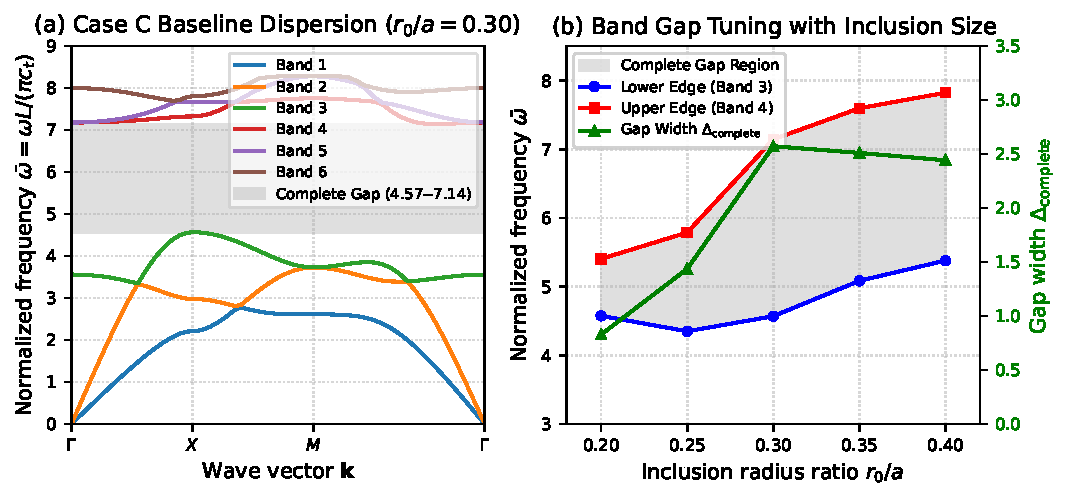
\includegraphics[width=\textwidth]{figures/fig07_caseC_dispersion.pdf}
\caption{Case-C dispersion on the $4\times4$ mesh. (a) Bands~3--4 gap at $r_0/L=0.30$. (b) Gap width versus inclusion radius. The width is not mesh-converged.}
\label{fig:caseC_dispersion}
\end{figure*}

Under mesh refinement, the complete gap falls from $2.5732$ at $4\times4$ to $2.2504$, $2.0722$, $1.9736$, and $1.9179$ at $8\times8$, $16\times16$, $32\times32$, and $64\times64$, respectively. The gap remains open on all five meshes, but its width has not converged. In particular, $2.5732$ describes the $4\times4$ calculation, not the continuum limit. At the $4\times4$ mesh, increasing $r_0/L$ from $0.20$ to $0.30$ widens the gap from $0.8288$ ($16.61\%$) to $2.5732$ ($43.94\%$); it then narrows to $2.4426$ ($37.00\%$) at $r_0/L=0.40$. Mesh and Brillouin-zone sampling details are reported in Appendix~\ref{app:caseC_resolution}.

\subsection{Group-velocity steering}
\label{sec:steering}
On the constant-wavenumber ring $|\bmk|=\bar{k}=0.5$, anisotropy makes the group velocity non-collinear with the wave vector. Group velocity is normal to the local constant-frequency contour because $\bmv_g=\nabla_{\bmk}\omega$. Its angle relative to $\bmk$ therefore depends on the contour slope. Figure~\ref{fig:ifc_wave_steering} plots the angular deviation $\delta(\phi)=\angle\bmv_g-\angle\bmk$ and group-velocity magnitude at $\theta=45^\circ$. The peak deviation rises from $0^\circ$ at $\mathrm{AR}=1$ to $1.4146^\circ$ at $\mathrm{AR}=5$ and $2.7846^\circ$ at $\mathrm{AR}=10$. The magnitude $|\bmv_g|$ also varies around the contour, so the anisotropic dispersion changes the energy-transport speed as well as its direction.

\begin{figure*}[htbp]
\centering
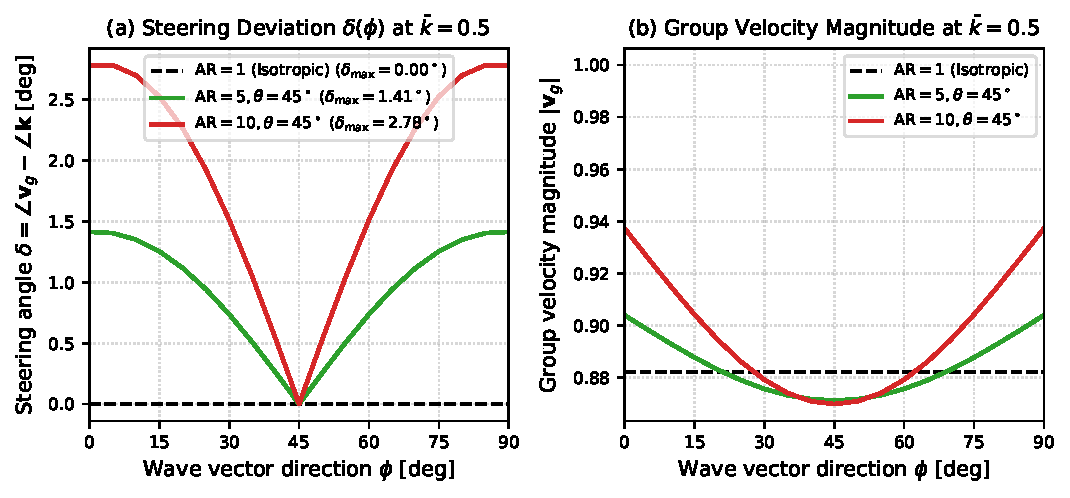
\includegraphics[width=\textwidth]{figures/fig12_ifc_wave_steering.pdf}
\caption{Acoustic-branch group-velocity steering on $|\bmk|=0.5$ at $\theta=45^\circ$. (a) Angular deviation for $\mathrm{AR}=1,5,10$, with peak values $0^\circ$, $1.4146^\circ$, and $2.7846^\circ$. (b) Directional variation of group-velocity magnitude}
\label{fig:ifc_wave_steering}
\end{figure*}

The orientation sweep uses $\theta=0^\circ,15^\circ,\ldots,90^\circ$ at $\mathrm{AR}=5$ and $10$ (Figure~\ref{fig:s7_steering_sweep}; Table~\ref{tab:steering_sweep}). Directions on the wavenumber ring are sampled every $5^\circ$, and a local parabola refines the estimated peak. The refined peaks vary by less than $10^{-5}\,$deg around $1.4146^\circ$ and $2.7846^\circ$, respectively. This small variation reflects the numerical procedure; it should not be interpreted as physical angular accuracy to $10^{-5}$ degrees. The principal direction follows $\phi^*(\theta)\simeq(45^\circ-\theta)\bmod90^\circ$; at $\mathrm{AR}=10$, its excursions are at most $5^\circ$. For the branch and wavenumber ring examined, tensor rotation mainly changes the steering direction. It has little effect on the sampled maximum deviation.

\begin{figure*}[htbp]
\centering
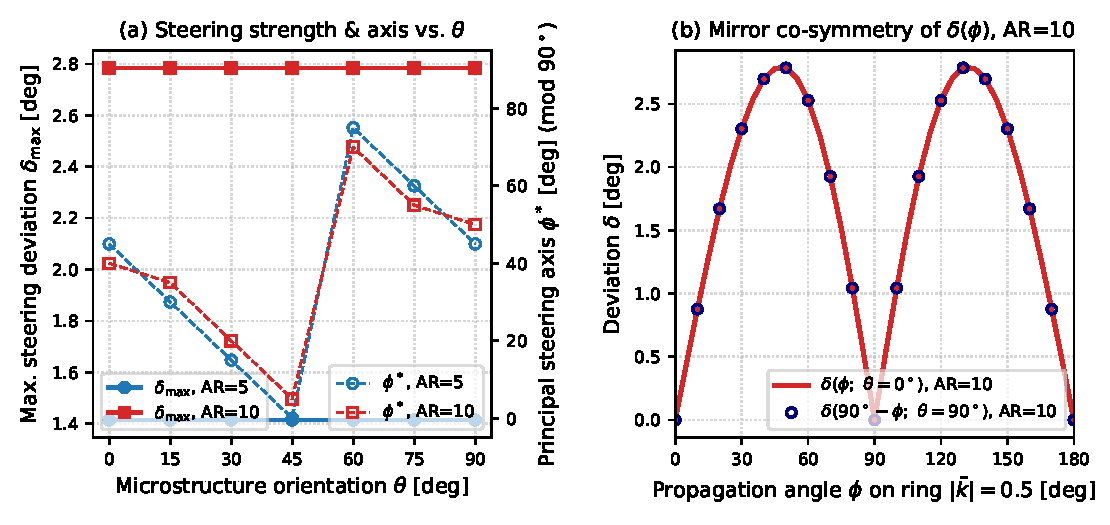
\includegraphics[width=\textwidth]{figures/fig14_s7_steering_sweep.pdf}
\caption{Orientation-dependent steering on $|\bmk|=0.5$. (a) Peak deviation and lobe direction for $\mathrm{AR}=5,10$. (b) Mirrored deviation fields at $\theta=0^\circ$ and $90^\circ$.}
\label{fig:s7_steering_sweep}
\end{figure*}

\begin{table}[htbp]
\centering
\caption{Peak group-velocity deviation and principal steering direction across the sampled orientations at $\bar{k}=0.5$}
\label{tab:steering_sweep}
\setlength{\tabcolsep}{4.5pt}%
\begin{tabular*}{\textwidth}{@{\extracolsep{\fill}}c r r r r@{}}
\toprule
$\theta$ & \multicolumn{2}{c}{$\mathrm{AR}=5$} & \multicolumn{2}{c}{$\mathrm{AR}=10$} \\
\cmidrule(lr){2-3}\cmidrule(lr){4-5}
 & $\delta_{\max}$ [deg] & $\phi^*$ [deg] & $\delta_{\max}$ [deg] & $\phi^*$ [deg] \\
\midrule
$0^\circ$ & 1.4146 & 45 & 2.7846 & 40 \\
$15^\circ$ & 1.4146 & 30 & 2.7846 & 35 \\
$30^\circ$ & 1.4146 & 15 & 2.7846 & 20 \\
$45^\circ$ & 1.4146 & 0 & 2.7846 & 5 \\
$60^\circ$ & 1.4146 & 75 & 2.7846 & 70 \\
$75^\circ$ & 1.4146 & 60 & 2.7846 & 55 \\
$90^\circ$ & 1.4146 & 45 & 2.7846 & 50 \\
\bottomrule
\end{tabular*}
\par\vspace{2pt}\begin{minipage}{\textwidth}\footnotesize $M_s=\phi^*(90^\circ)-\phi^*(0^\circ)$: $M_s(\mathrm{AR}=5)=0^\circ$ and $M_s(\mathrm{AR}=10)=10^\circ$. The $5^\circ$ ring-sampling step limits the resolution of this difference; parabolic peak refinement remains within one sampling step.\end{minipage}
\par\vspace{2pt}\begin{minipage}{\textwidth}\footnotesize Headless periodicity and mirror co-symmetry residuals are each $\le1.3\times10^{-6}\,$deg: $\delta(\phi;\theta)=\delta(\phi+180^\circ;\theta)$ and $\delta(\phi;\theta)=\delta(90^\circ-\phi;90^\circ-\theta)$.\end{minipage}

\end{table}

We define the sampled steering measure as follows:
\begin{equation}
M_s(\mathrm{AR})=\phi^*(90^\circ,\mathrm{AR})-\phi^*(0^\circ,\mathrm{AR}),
\label{eq:Ms_def}
\end{equation}
For the two aspect ratios, the values are:
\begin{equation}
M_s(\mathrm{AR}=5)=0^\circ,\qquad M_s(\mathrm{AR}=10)=10^\circ.
\label{eq:Ms_value}
\end{equation}
The $5^\circ$ ring-sampling step sets the resolution of this difference. The deviation field is headless-periodic and mirror co-symmetric, with residuals no greater than $1.3\times10^{-6}\,$deg. The peak amplitude is invariant under $\theta\mapsto90^\circ-\theta$ to within $10^{-7}\,$deg. These symmetries are consistent with orientation shifting the lobes while leaving the sampled peak deviation unchanged.
